%%%%%%%%%%%%%%%%%%%%%%%%%%%%%%%%%%%%%%%%%
% Beamer Presentation
% LaTeX Template
% Version 1.0 (10/11/12)
%
% This template has been downloaded from:
% http://www.LaTeXTemplates.com
%
% License:
% CC BY-NC-SA 3.0 (http://creativecommons.org/licenses/by-nc-sa/3.0/)
%
%%%%%%%%%%%%%%%%%%%%%%%%%%%%%%%%%%%%%%%%%

%----------------------------------------------------------------------------------------
%	PACKAGES AND THEMES
%----------------------------------------------------------------------------------------

% \documentclass{beamer}
\documentclass[handout]{beamer}

\mode<presentation> {

\usetheme{Madrid}

}

\definecolor{DataBlue}{rgb}{0.50, 0.85, 0.99} 

\setbeamercolor{titlelike}{parent=structure,bg=black, fg = white}
\setbeamercolor{frametitle}{fg=white}
\usepackage{graphicx} % Allows including images
\usepackage{booktabs} % Allows the use of \toprule, \midrule and \bottomrule in tables
\usepackage[export]{adjustbox}
\usepackage[portuguese]{babel}
\usepackage[utf8]{inputenc}

\usepackage{pgfplots}
\usepackage{tikz}
\usetikzlibrary{calc,babel,quotes,angles}
\usepackage{tkz-euclide}

\usepackage{amsmath, amsfonts, amssymb}

\usepackage{multirow}
% \usepackage{xcolor}

\makeatletter
\let\save@measuring@true\measuring@true
\def\measuring@true{%
  \save@measuring@true
  \def\beamer@sortzero##1{\beamer@ifnextcharospec{\beamer@sortzeroread{##1}}{}}%
  \def\beamer@sortzeroread##1<##2>{}%
  \def\beamer@finalnospec{}%
}
\makeatother


%----------------------------------------------------------------------------------------
%	TITLE PAGE
%----------------------------------------------------------------------------------------

\title{Geometria} %% Title
\author{Gustavo Ale} % Your name
\institute[UFMT] % Your institution as it will appear on the bottom of every slide, may be shorthand to save space
{
EduCursinho - Faculdade de Engenharia \\ % Your institution for the title page
\medskip
\textit{gustavo.engca@gmail.com} % Your email address
}
\date{\today} % Date, can be changed to a custom date

% Rodapé
% \setbeamertemplate{footline}{%
%     \begin{beamercolorbox}[wd=\paperwidth]{footlinecolor}
%         \includegraphics[width=\paperwidth]{images/footbar.png}
%     \end{beamercolorbox}%
% }

\begin{document}
{
\setbeamertemplate{footline}{}
\begin{frame}
    \begin{columns}
        \begin{column}{0.48\textwidth}
            % \hspace*{-1cm}
            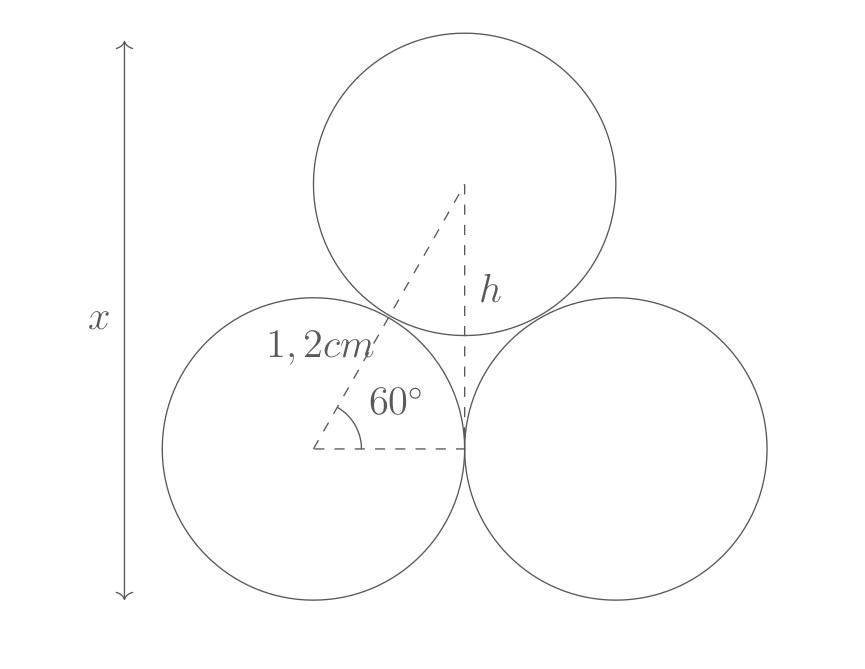
\includegraphics[width=\columnwidth,left]{../assets/geo.png}
        \end{column}
        \begin{column}{0.48\textwidth}
            \titlepage
        \end{column}
    \end{columns}

\end{frame}
}

%-------------------------------------------------------------------------------
% Sumário
%-------------------------------------------------------------------------------

\begin{frame}
    \frametitle{Sumário} % Table of contents slide, comment this block out to remove it
    \tableofcontents % Throughout your presentation, if you choose to use \section{} and \subsection{} commands, these will automatically be printed on this slide as an overview of your presentation
\end{frame}

%----------------------------------------------------------------------------------------
%	PRESENTATION SLIDES
%----------------------------------------------------------------------------------------

\section{Geometria}
\subsection{O que é geometria}
\begin{frame}\frametitle{\subsecname}
    A geometria é provavelmente a área mais antiga da matemática, precursora da própria álgebra e sendo um dos pilares
    da matemática. A palavra geometria é resultado da combinação das palavras gregas \textit{geo} e
    \textit{metron}/\textit{metri}, significando respectivamente Terra e medição, pois a área da geometria consiste da
    medição e entendimento das relações e propriedades  contidas nas fíguras geométricas: comprimento, distância, ângulo,
    área, volume e perímetro, as fíguras geométricas por sua vez são parte integrante da natureza e da Terra (\textit{geo}).
\end{frame}

%------------------------------------------------

\subsection{Definições gerais}
\begin{frame}\frametitle{\subsecname}
    Antes do estudo da geometria devemos ter ciência das definições de conceitos presentes nesse ramo da matemática,
    dentro destes conceitos se enquadram as medidas, os ângulos, as fíguras geométricas e suas componentes:
    \begin{itemize}
        \item comprimento, raio, circunferência
        \item área
        \item volume
        \item ângulo
    \end{itemize}
\end{frame}

%------------------------------------------------

\subsection{Distância e comprimento}
\begin{frame}\frametitle{\subsecname}
    Distância e comprimento medem o quão longe dois pontos estão entre si, e no caso de arestas essa medida é
    denotada como comprimento. A unidade de medida base utilizada para comprimento é o metro (símbolo ${m}$), além do
    metro existem seus múltiplos que são igualmente utilizados dependendo da distância/comprimento aferido.

    \begin{figure}[H]
        \centering
        %\resizebox{\columnwidth}{!}
        \caption{$d$ representa a distância entre os pontos que formam a reta $\overline{AB}$}
    \end{figure}

\end{frame}

%------------------------------------------------

\begin{frame}\frametitle{\subsecname}
    \begin{table}[H]
        \resizebox{0.5\textwidth}{!}{%
            \begin{tabular}{l|l|l}
                \textbf{Nome} & \textbf{Sigla} & \textbf{Equivalência} \\ \hline
                picometro     & $pm$           & $10^{-12}m$           \\
                nanometro     & $nm$           & $10^{-9}m$            \\
                micrometro    & $\mu m$        & $10^{-6}m$            \\
                milimetro     & $mm$           & $10^{-3}m$            \\
                centímetro    & $cm$           & $10^{-2}m$            \\
                decímetro     & $dm$           & $10^{-1}m$            \\
                metro         & $m$            & $1m$                  \\
                decâmetro     & $dam$          & $10m$                 \\
                hêctometro    & $hm$           & $100m$                \\
                quilometro    & $km$           & $1000m$
            \end{tabular}%
        }
        %\caption{Unidades medida de comprimento e distância}
    \end{table}
\end{frame}

%------------------------------------------------

\begin{frame}\frametitle{\subsecname}
    \begin{columns}
        \column{0.45\textwidth}
        \begin{figure}[H]
            \centering
            %\resizebox{\columnwidth}{!}
            \caption{Raio $r$, diâmetro $d$ e circunferência $c$ de um círculo}
        \end{figure}

        A circunferência do círculo é $2\pi r$.

        \column{0.5\textwidth}
        \begin{block}{Perímetro}
            comprimento do contorno de uma fígura geométrica. \\
        \end{block}

        \begin{block}{Raio}
            distância entre o centro de uma circunferência até seu contorno ou superfície.
        \end{block}

        \begin{block}{Diâmetro}
            comprimento de reta que passe pelo centro da circunferência e cujo seus pontos de início e fim estejam sobre a circunferência
        \end{block}

        % \begin{block}{Circunferência}
        %     perímetro de uma circunferência.
        % \end{block}

    \end{columns}

\end{frame}

%------------------------------------------------

\subsection{Área}
\begin{frame}\frametitle{\subsecname}
    Área é a medida que expressa a quantidade de espaço bidimenssional ocupado por uma fígura geométrica. A unidade base
    para área é o \textbf{metro quadrado (símbolo ${m^2}$)}. Seus múltiplos também acompanham o termo 'quadrado',
    e a equivalência é a mesma do metro, porém elevada ao quadrado.
    \pause Ex.:

    \begin{align*}
        1m   & = 100cm     \\
        \pause
        1m^2 & = (100cm)^2 \\
        \pause
        1m^2 & = 100^2cm^2
    \end{align*}

\end{frame}

%------------------------------------------------

\begin{frame}\frametitle{\subsecname}

    \begin{figure}[H]
        \centering
        %\resizebox{\columnwidth}{!}{%
        \begin{tikzpicture}
            \coordinate (A) at (0,0);
            \coordinate (B) at (4,3);
            \coordinate (C) at (4,0);
            % \coordinate (D) at (0,3);
            \node[circle, fill, label={left:$A$}, inner sep=2pt] at (A) {};
            \node[circle, fill, label={right:$B$}, inner sep=2pt] at (B) {};
            \node[circle, fill, label={right:$C$}, inner sep=2pt] at (C) {};
            % \node[circle, fill, label={left:$D$}, inner sep=2pt] at (D) {};
            % \draw[dashed] (A)--(D)--(B);
            \draw[fill=gray!25] (A)--(B)--(C)--(A);
        \end{tikzpicture}
        %}
        \caption{Área é o espaço bidimenssional ocupado pela região cinza.}
        \label{fig:tri_abc}
    \end{figure}
\end{frame}

%------------------------------------------------

\begin{frame}\frametitle{\subsecname}

    \begin{table}[H]
        \resizebox{0.5\columnwidth}{!}{%
            \begin{tabular}{l|l|l}
                \textbf{Nome}       & \textbf{Sigla} & \textbf{Equivalência}       \\ \hline
                picometro quadrado  & $pm^2$         & $10^{-24}m^2$               \\
                nanometro quadrado  & $nm^2$         & $10^{-18}m^2$               \\
                micrometro quadrado & $\mu m$        & $10^{-12}m^2$               \\
                milimetro quadrado  & $mm^2$         & $10^{-6}m^2$                \\
                centímetro quadrado & $cm^2$         & $10^{-4}m^2$                \\
                decímetro quadrado  & $dm^2$         & $10^{-2}m^2$                \\
                metro quadrado      & $m^2$          & $1m^2$                      \\
                decâmetro quadrado  & $dam^2$        &                             \\
                are                 & $are$          & \multirow{-2}{*}{$100m^2$}  \\
                hêctometro quadrado & $hm^2$         &                             \\
                hectare             & $ha$           & \multirow{-2}{*}{$10^4m^2$} \\
                quilometro quadrado & $km^2$         & $10^6m^2$
            \end{tabular}%
        }
        %\caption{Unidades medida de área}
    \end{table}
\end{frame}

%------------------------------------------------

\subsection{Volume}

\begin{frame}\frametitle{\subsecname}
    O volume expressa
    a quantidade de espaço tridimenssional ocupado por um objeto. No caso do volume existe duas unidades de medida base,
    o \textbf{metro cúbico (símbolo $m^3$)} e o \textbf{litro}, ambos são usados regularmente, na qual o litro é a unidade mais usada para volumes
    pequenos, enquanto o metro cúbico é usado para expressar volumes maiores.

    \begin{align*}
        1m   & = 100cm     \\
        \pause
        1m^3 & = (100cm)^3 \\
        \pause
        1m^3 & = 100^3cm^3
    \end{align*}
\end{frame}

%------------------------------------------------

\begin{frame}\frametitle{\subsecname}
    \begin{figure}[H]
        \centering
        %\resizebox{0.5\columnwidth}{!}{%
        \begin{tikzpicture}
            \coordinate (A) at (0,0);
            \coordinate (B) at (0,3);
            \coordinate (C) at (3,3);
            \coordinate (D) at (3,0);
            \coordinate (E) at (1,1);
            \coordinate (F) at (1,4);
            \coordinate (G) at (4,4);
            \coordinate (H) at (4,1);
            \draw[fill=gray!25] (A)--(B)--(F)--(G)--node[right]{$L$}(H)--node[right]{$L$}(D)--node[below]{$L$}(A);
            \draw (B)--(C)--(D);
            \draw (C)--(G);
            \draw[dashed] (A)--(E)--(H);
            \draw[dashed] (E)--(F);
        \end{tikzpicture}
        %}
        \caption{Cubo, cujo volume se dá por $L^3$, onde $L$ é o comprimento das arestas}
    \end{figure}
\end{frame}

%------------------------------------------------

\begin{frame}\frametitle{\subsecname}
    \begin{table}[H]
        \resizebox{0.5\columnwidth}{!}{%
            \begin{tabular}{l|l|l}
                \textbf{Nome}     & \textbf{Sigla} & \textbf{Equivalência}          \\ \hline
                milimetro cúbico  & $mm^3$         & $10^{-9}m^3$                   \\ \hline
                centímetro cúbico & $cm^3$         &                                \\
                mililitro         & $ml$           & \multirow{-2}{*}{$10^{-6}m^3$} \\ \hline
                decímetro cúbico  & $dm^3$         &                                \\
                litro             & $l$            & \multirow{-2}{*}{$10^{-3}m^3$} \\ \hline
                metro cúbico      & $m^3$          & $1m^2$                         \\ %\hline                      
            \end{tabular}%
        }
        %\caption{Unidades medida de volume}
    \end{table}
\end{frame}

%------------------------------------------------
\subsection{Ângulo}

\begin{frame}\frametitle{\subsecname}
    Ângulo é uma medida de inclinação entre duas retas ou dois planos, desde que eles não sejam paralelos entre si, no
    contexto da geometria os ângulos estão presentes em todos os vértices das fíguras geométricas.
    As unidades de medida mais comuns para ângulo são \textbf{graus} (símbolo $^{\circ}$), \textbf{radianos} (símbolo $rad$) e \textbf{gradianos} (símbolo $gon$).

    Quanto no escopo das funções trigonométricas a unidade de medida mais utilizada é o radiano, por outro lado,
    em aplicações de engenharia e na geometria a unidade mais usada é o grau. Considerando um grau $\alpha$ em graus,
    sua conversão para radianos se dá por $rad(\alpha) = \alpha\cdot\pi/180$

\end{frame}

%------------------------------------------------

\begin{frame}[fragile]\frametitle{\subsecname}
    \begin{figure}[H]
        \centering
        %\resizebox{\columnwidth}{!}{%
        \begin{tikzpicture}
            \coordinate (O) at (1,2);
            \coordinate (A) at (0.5,1);
            \coordinate (B) at (2.5,5);
            \coordinate (C) at (0,2);
            \coordinate (D) at (5,2);
            \draw (A)--(B) node[above] {$p$};
            \draw (C)--(D) node[above] {$q$};
            % \draw (O) node[above right] {$65^\circ$};
            % \pic[angle radius=1cm,"$\alpha$"] {angle=a--b--c};
            \pic ["$65^\circ$", draw, -, angle eccentricity=2] {angle = D--O--B};
            % \draw (B)--(C);
            % \draw (A)--(C);
        \end{tikzpicture}
        %}
        \caption{Ângulo entre as retas $p$ e $q$}
    \end{figure}
\end{frame}

%------------------------------------------------

\begin{frame}[fragile]\frametitle{\subsecname}
    Uma reta $p$ é \textbf{perpendicular} a reta $q$ se o ângulo formado entre elas for de 90 graus.
    \begin{figure}[H]
        \centering
        %\resizebox{\columnwidth}{!}{%
        \begin{tikzpicture}
            \coordinate (O) at (1,1.5);
            \coordinate (A) at (0,2);
            \coordinate (B) at (4,0);
            \coordinate (C) at (0,0);
            \coordinate (D) at (3,4.5);
            \draw (A)--(B) node[above] {$p$}  ;
            \draw (C)--(D) node[left] {$q$};
            % \pic[angle radius=1cm,"$\alpha$"] {angle=a--b--c};
            \pic ["$90^{\circ}$", draw, -, angle eccentricity=2] {angle = B--O--D};
            % \draw (B)--(C);
            % \draw (A)--(C);
        \end{tikzpicture}
        %}
        \caption{Retas perpendiculares $p$ e $q$}
    \end{figure}
\end{frame}

%------------------------------------------------

\begin{frame}[fragile]\frametitle{\subsecname}
    Duas retas $p$ e $q$ são consideradas \textbf{paralelas entre si}, se qualquer reta $r$ perpendicular a reta $p$ também for
    perpendicular a reta $q$. Outra forma de descrever retas paralelas é através do \textbf{Quinto Postulado de Euclides}
    que diz: Supondo que duas retas $p$ e $q$ são cortadas por uma terceira reta $r$. Se a soma dos ângulos formados um
    mesmo lado da reta $r$ resultar em 180 graus, então $m$ e $n$ são retas paralelas entre si.

    \begin{figure}[H]
        \centering
        %\resizebox{\columnwidth}{!}
        \caption{Retas paralelas $p$ e $q$}
    \end{figure}
\end{frame}

%------------------------------------------------

\subsection{Exercícios}
\begin{frame}\frametitle{\subsecname}
    \begin{block}{Exercícios}
        Converta:
        \begin{itemize}
            \item a) $1903m$ para $mm$
            \item b) $17km$ para $m$
            \item c) $10cm^3$ para $dm^3$
            \item d) $20L$ para $m^3$
            \item e) $2ha$ para $m^2$
            \item f) $2\pi$ para graus
        \end{itemize}
    \end{block}
\end{frame}

%------------------------------------------------

\begin{frame}
    \Huge{\centerline{Perguntas?}}
\end{frame}

%----------------------------------------------------------------------------------------

\end{document}